\documentclass{article}
\usepackage[utf8]{inputenc}
\usepackage[T2A]{fontenc}
\usepackage[english,russian]{babel}
\usepackage{indentfirst}
\usepackage[a4paper, top = 1.5cm, bottom=1.5cm,left=2cm,right=1cm]{geometry}
\usepackage{amsmath}
\usepackage{amsfonts}
\usepackage{graphicx}
\usepackage{wrapfig}
\usepackage{hyperref}


%\usepackage{biblatex} 
%\addbibresource{biblio_jebref.bib}


\setlength{\parindent}{0.1ex}
%\setlength{\parskip}{0.2em}


\title{Марковские Цепи}
\author{Саттаров Никита, 322 гр.}
\date{October 2020}

\begin{document}
\maketitle

%\newcommand{\anonsection}[1]{\section*{#1}\addcontentsline{toc}{section}{#1}}
%\newcommand{\anonsubsection}[1]{\subsection*{#1}\addcontentsline{toc}{subsection}{#1}}
%\newcommand{\anonsubsubsection}[1]{\subsubsection*{#1}\addcontentsline{toc}{subsubsection}{#1}}
	\newcommand{\ds}{\displaystyle}

{\bfseries Цепь Маркова}  ---  последовательность случайных событий с конечным или счётным числом исходов, где вероятность наступления каждого события зависит от состояния, достигнутого в предыдущем событии. Характеризуется тем свойством, что, говоря нестрого, при фиксированном настоящем будущее независимо от прошлого. Названа в честь А. А. Маркова (старшего), который впервые ввёл это понятие в работе 1906 года.\\
$\sum\limits_{0}^{\lfloor \frac{k}{3} \rfloor}{v}$
\tableofcontents

\section{Цепь Маркова с дискретным временем}

\subsection{Определение}
\begin{wrapfigure}[10]{r}{0.25\textwidth}
	\begin{center}
		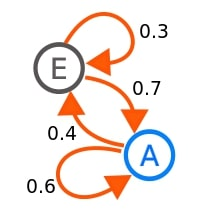
\includegraphics[width = 0.2\textwidth]{image_1.jpg}
	\end{center}
	\caption{Пример цепи с двумя состояниями}
\end{wrapfigure}
Последовательность дискретных случайных величин ${\ds \{X_{n}\}_{n \geq 0} }$ называется простой цепью Маркова (с дискретным временем), если

\begin{equation*}
	\mathbb{P}(X_{n+1}=i_{n+1} \mid X_{n} = i_{n}, X_{n-1} = i_{n-1}, \ldots , X_{0} = i_{0}) = \mathbb{P} (X_{n+1}=i_{n+1} \mid X_{n} = i_{n}).
\end{equation*}

Таким образом, в простейшем случае условное распределение последующего состояния цепи Маркова зависит только от текущего состояния и не зависит от всех предыдущих состояний (в отличие от цепей Маркова высших порядков).

Область значений случайных величин ${\ds \{X_{n}\} }$ называется {\bfseries пространством состояний} цепи, а номер $n$ — номером шага.

\subsection{Переходная матрица и однородные цепи}
Матрица ${\ds P(n)}$, где

\begin{equation*}
	P_{ij}(n) \equiv \mathbb {P}(X_{n+1} = j \mid X_{n}=i)
\end{equation*}

называется {\bfseries матрицей переходных вероятностей} на $n$-м шаге, а вектор ${\ds\mathbf{p} = (p_{1},p_{2},\ldots )^{\top }}$, где

\begin{equation*}
	p_{i} \equiv \mathbb  {P} (X_{0} = i)
\end{equation*}

"--* {\bfseries начальным распределением} цепи Маркова.

Очевидно, матрица переходных вероятностей является стохастической, то есть

\begin{equation*}
	\sum_{j} P_{ij}(n) = 1, \quad \forall n \in {\mathbb{N}}.
\end{equation*}

Цепь Маркова называется {\bfseries однородной}, если матрица переходных вероятностей не зависит от номера шага, то есть

\begin{equation*}
	P_{ij}(n)=P_{ij},\quad \forall n\in {\mathbb{N}}.
\end{equation*}

В противном случае цепь Маркова называется неоднородной. В дальнейшем будем предполагать, что имеем дело с однородными цепями Маркова.

\subsection{Конечномерные распределения и матрица перехода за n шагов}
Из свойств условной вероятности и определения однородной цепи Маркова получаем:

\begin{equation*}
	{\mathbb  {P}}(X_{n}=i_{n},\ldots ,X_{0}=i_{0})=P_{i_{{n-1},i_{n}}} \cdots P_{{i_{0},i_{1}}}P_{{i_{0}}},
\end{equation*}

откуда вытекает специальный случай уравнения Колмогорова — Чепмена:

\begin{equation*}
	{\mathbb  {P}}(X_{n}=i_{n}\mid X_{0}=i_{0})=(P^{n})_{{i_{0},i_{n}}}, 
\end{equation*}

то есть матрица переходных вероятностей за $n$ шагов однородной цепи Маркова есть $n$-я степень матрицы переходных вероятностей за 1 шаг. Наконец,

\begin{equation*}
	{\mathbb  {P}}(X_{n}=i_{n})=\left((P^{T})^{n}{\mathbf  {p}}\right)_{{i_{n}}}.
\end{equation*}

\subsection{Типы состояний}
	\begin{itemize}
		\item Возвратное состояние.
		\item Возвратная цепь Маркова.
		\item Достижимое состояние.
		\item Неразложимая цепь Маркова.
		\item Периодическое состояние.
		\item Периодическая цепь Маркова.
		\item Поглощающее состояние. Состояние $i$ называется поглощающим если $P_{i,i}=1$.
		\item Эргодическое состояние.
	\end{itemize}

\subsection{Примеры}
\begin{itemize}
	\item Ветвящийся процесс;
	\item Случайное блуждание;
\end{itemize}

\section{Цепь Маркова с непрерывным временем}

\subsection{Определение}
Семейство дискретных случайных величин ${\ds\{X_{t}\}_{t\geq 0}}$ называется цепью Маркова (с непрерывным временем), если

\begin{equation*}
	{\mathbb  {P}}(X_{{t+h}}=x_{{t+h}}\mid X_{s}=x_{s},\;0<s\leq t)={\mathbb  {P}}(X_{{t+h}}=x_{{t+h}}\mid X_{t}=x_{t}).
\end{equation*}

Цепь Маркова с непрерывным временем называется однородной, если

\begin{equation*}
	{\mathbb  {P}}(X_{{t+h}}=x_{{t+h}}\mid X_{t}=x_{t})={\mathbb  {P}}(X_{{h}}=x_{{h}}\mid X_{0}=x_{0}).
\end{equation*}

\subsection{Матрица переходных функций и уравнение Колмогорова "--~ Чепмена}
Аналогично случаю дискретного времени, конечномерные распределения однородной цепи Маркова с непрерывным временем полностью определены начальным распределением

\begin{equation*}
	{\mathbf  {p}}=(p_{1},p_{2},\ldots )^{{\top }},\;p_{i}={\mathbb  {P}}(X_{0}=i),\quad i=1,2,\ldots 
\end{equation*}

и {\bfseries матрицей переходных функций} (\textit{переходных вероятностей})

\begin{equation*}
	{\mathbf  {P}}(h)=(P_{{ij}}(h))={\mathbb  {P}}(X_{h}=j\mid X_{0}=i). 
\end{equation*}

Матрица переходных вероятностей удовлетворяет уравнению Колмогорова — Чепмена: ${ds\mathbf {P} (t+s)=\mathbf {P} (t)\mathbf {P} (s)}$ или

\begin{equation*}
	P_{{ij}}(t+s)=\sum _{k}P_{{ik}}(t)P_{{kj}}(s). 
\end{equation*}

\subsection{Матрица интенсивностей и дифференциальные уравнения Колмогорова}
По определению, матрица интенсивностей ${\ds \mathbf {Q} =\lim _{h\to 0}{\frac {\mathbf {P} (h)-\mathbf {I} }{h}}}$ или, что эквивалентно,

\begin{equation*}
	{\mathbf  {Q}}=(q_{{ij}})=\left({\frac  {dP_{{ij}}(h)}{dh}}\right)_{{h=0}}. 
\end{equation*}

Из уравнения Колмогорова — Чепмена следуют два уравнения:

\begin{itemize}
	\item Прямое уравнение Колмогорова
	
	\begin{equation*}
		{\frac  {d{\mathbf  {P}}(t)}{dt}}={\mathbf  {P}}(t){\mathbf  {Q}},
	\end{equation*}
	
	\item Обратное уравнение Колмогорова
	
	\begin{equation*}
		{\frac  {d{\mathbf  {P}}(t)}{dt}}={\mathbf  {Q}}{\mathbf  {P}}(t). 
	\end{equation*}
\end{itemize}

Для обоих уравнений начальным условием выбирается ${\ds \mathbf {P} (0)=\mathbf {I} }$. Соответствующее решение ${\ds \mathbf {P} (t)=\exp(\mathbf {Q} t).}$.

\subsection{Свойства матриц P и Q}

Для любого ${\ds t>0}$ матрица ${\ds \mathbf {P} (t)}$ обладает следующими свойствами:

\begin{enumerate}
	\item Матричные элементы ${\ds \mathbf {P} (t)}$ неотрицательны: ${\ds P_{ij}(t)\geq 0}$ (неотрицательность вероятностей).	
	\item Сумма элементов в каждой строке ${\ds \mathbf {P} (t)}$ равна 1: ${\ds \sum _{j}P_{ij}(t)=1}$ (полная вероятность), то есть матрица ${\ds \mathbf {P} (t)}$ является стохастической справа (или по строкам).
	\item Все собственные числа ${\ds \lambda }$  матрицы ${\ds \mathbf {P} (t)}$ не превосходят 1 по абсолютной величине: ${\ds |\lambda |\leq 1}$. Если ${\ds |\lambda |=1}$S, то ${\ds \lambda =1}$.
	\item Собственному числу ${\ds \lambda =1}$ матрицы ${\ds \mathbf {P} (t)}$ соответствует, как минимум, один неотрицательный левый собственный вектор-строка (равновесие): ${\ds (p_{1}^{*},\,p_{2}^{*},...); p_{i}^{*}\geq 0; \sum _{i}p_{i}^{*}=1; \sum _{i}p_{i}^{*}P_{ij}(t)=p_{j}^{*}}$.
	\item Для собственного числа ${\ds \lambda =1}$ матрицы ${\ds \mathbf {P} (t)}$ все корневые векторы являются собственными, то есть соответствующие жордановы клетки тривиальны.
\end{enumerate}

Матрица ${\ds \mathbf {Q} }$ обладает следующими свойствами:

\begin{enumerate}
	\item Внедиагональные матричные элементы ${\ds \mathbf {Q} }$ неотрицательны: ${\ds q_{ij}\geq 0\;i\neq j}$.
	\item Диагональные матричные элементы ${\ds \mathbf {Q} }$ неположительны: ${\ds q_{ii}\leq 0}$.
	\item Сумма элементов в каждой строке ${\ds \mathbf {Q} }$ равна 0: ${\ds \sum _{j}q_{ij}=0}$.
	\item Действительная часть всех собственных чисел ${\ds \mu }$  матрицы ${\ds \mathbf {Q} }$ неположительна: ${\ds Re(\mu )\leq 0}$. Если ${\ds Re(\mu )=0}$, то ${\ds \mu =0}$.
	\item Собственному числу ${\ds \mu =0}$ матрицы ${\ds \mathbf {Q} }$ соответствует, как минимум, один неотрицательный левый собственный вектор-строка (равновесие): ${\ds (p_{1}^{*},\,p_{2}^{*},...); p_{i}^{*}\geq 0; \sum _{i}p_{i}^{*}=1; \sum _{i}p_{i}^{*}q_{ij}=0}$.
	\item Для собственного числа ${\ds \mu =0}$ матрицы ${\ds \mathbf {Q} }$ все корневые векторы являются собственными, то есть соответствующие жордановы клетки тривиальны.
\end{enumerate}

\subsection{Граф переходов, связность и эргодические цепи Маркова}
Для цепи Маркова с непрерывным временем строится ориентированный граф переходов (кратко "--- граф переходов) по следующим правилам:

\begin{itemize}
	\item Множество вершин графа совпадает со множеством состояний цепи.
	\item Вершины ${\ds i,j\,(i\neq j)}$ соединяются ориентированным ребром ${\ds i\to j}$, если ${\ds q_{ij}>0}$ (то есть интенсивность потока из ${\ds i}$-го состояния в ${\ds j}$-е положительна.
\end{itemize}

Топологические свойства графа переходов связаны со спектральными свойствами матрицы ${\ds \mathbf {Q} }$. В частности, для конечных цепей Маркова верны следующие теоремы:

\begin{itemize}
	\item Следующие три свойства $1, 2, 3$ конечной цепи Маркова эквивалентны (обладающие ими цепи иногда называют \textbf{слабо эргодическими}):
	\begin{enumerate}
		\item Для любых двух различных вершин графа переходов ${\ds i,j\,(i\neq j)}$ найдется такая вершина $k$ графа («общий сток»), что существуют ориентированные пути от вершины $i$ к вершине $k$ и от вершины $j$ к вершине $k$.\\
		\textit{Замечание}: возможен случай ${\ds k=i}$ или ${\ds e k=j}$; в этом случае тривиальный (пустой) путь от $i$ к $i$ или от $j$ к $j$ также считается ориентированным путём.
		\item Нулевое собственное число матрицы ${\ds \mathbf {Q} }$ невырождено.
		\item При ${\ds t\to \infty }$ матрица ${\ds \mathbf {P} (t)}$ стремится к матрице, у которой все строки совпадают (и совпадают, очевидно, с равновесным распределением).
	\end{enumerate}
	\item Следующие пять свойств $1, 2, 3, 4, 5$ конечной цепи Маркова эквивалентны (обладающие ими цепи называют \textbf{эргодическими}):
	\begin{enumerate}
		\item Граф переходов цепи ориентированно связен.
		\item Нулевое собственное число матрицы ${\ds \mathbf {Q} }$ невырождено и ему соответствует строго положительный левый собственный вектор (равновесное распределение).
		\item Для некоторого ${\ds t>0}$ матрица ${\ds \mathbf {P} (t)}$ строго положительна (то есть ${\ds P_{ij}(t)>0}$ для всех ${\ds i,j}$.
		\item Для всех ${\ds t>0}$ матрица ${\ds \mathbf {P} (t)}$ строго положительна.
		\item При ${\ds t\to \infty }$  матрица ${\ds \mathbf {P} (t)}$ стремится к строго положительной матрице, у которой все строки совпадают (и совпадают, очевидно, с равновесным распределением).
	\end{enumerate}
\end{itemize}

\subsection{Примеры}
\begin{wrapfigure}[10]{r}{0.35\textwidth}
	\begin{center}
		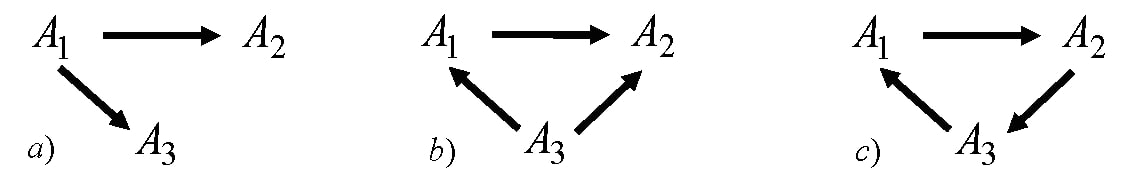
\includegraphics[width = 0.35\textwidth]{image_2.jpg}
	\end{center}
	\caption{Примеры графов переходов для цепей Маркова: a) цепь не является слабо эргодической (не существует общего стока для состояний ${\ds A_{2},\,A_{3}}$; b) слабо эргодическая цепь (граф переходов не является ориентированно связным) c) эргодическая цепь (граф переходов ориентированно связан).}
\end{wrapfigure}
Рассмотрим цепи Маркова с тремя состояниями и с непрерывным временем, соответствующие графам переходов, представленным на рис. 2. 
В случае (a) отличны от нуля только следующие недиагональные элементы матрицы интенсивностей "--- ${\ds q_{12},\,q_{13}}$, в случае (b) отличны от нуля только ${\ds q_{12},\,q_{31}\,q_{32}}$, а в случае (c) "--- ${\ds q_{12},\,q_{31}\,q_{23}}$. Остальные элементы определяются свойствами матрицы ${\ds \mathbf {Q} }$ (сумма элементов в каждой строке равна 0). В результате для графов (a), (b), (c) матрицы интенсивностей имеют вид: ${\ds \mathbf {Q} _{a}={\begin{pmatrix}-(q_{12}+q_{13})&q_{12}&q_{13}\\0&0&0\\0&0&0\end{pmatrix}}}$,\\
${\ds \mathbf {Q} _{b}={\begin{pmatrix}-q_{12}&q_{12}&0\\0&0&0\\q_{31}&q_{32}&-(q_{31}+q_{32})\end{pmatrix}}}$, ${\ds \mathbf {Q} _{c}={\begin{pmatrix}-q_{12}&q_{12}&0\\0&-q_{23}&q_{23}\\q_{31}&0&-q_{31}\end{pmatrix}}.}$

\section{Основное кинетическое уравнение}
\textbf{Основное кинетическое уравнение} описывает эволюцию распределения вероятностей в цепи Маркова с непрерывным временем. «Основное уравнение» здесь "--- не эпитет, а перевод термина англ. \textit{Master equation}. Для вектора-строки распределения вероятностей $\pi$  основное кинетическое уравнение имеет вид:

\begin{equation*}
	{\frac  {d\pi }{dt}}=\pi {\mathbf  {Q}}
\end{equation*}

и совпадает, по существу, с прямым уравнением Колмогорова. В физической литературе чаще используют векторы-столбцы вероятностей и записывают основное кинетическое уравнение в виде, который явно использует закон сохранения полной вероятности:

\begin{equation*}
	{\frac  {dp_{i}}{dt}}=\sum _{{j,\,j\neq i}}(T_{{ij}}p_{j}-T_{{ji}}p_{i}),
\end{equation*}

где ${\ds T_{ij}=q_{ji}.}$

Если для основного кинетического уравнения существует положительное равновесие ${\ds p_{i}^{*}>0}$, то его можно записать в форме:

\begin{equation*}
	{\frac  {dp_{i}}{dt}}=\sum _{{j,\,j\neq i}}T_{{ij}}p_{j}^{*}\left({\frac  {p_{j}}{p_{j}^{*}}}-{\frac  {p_{i}}{p_{i}^{*}}}\right).
\end{equation*}

\subsection{Функции Ляпунова для основного кинетического уравнения}
Для основного кинетического уравнения существует богатое семейство выпуклых функций Ляпунова "--- монотонно меняющихся со временем функций распределения вероятностей. Пусть ${\ds h(x)\,(x>0)}$ "--- выпуклая функция одного переменного. Для любого положительного распределения вероятностей $({\ds p_{i}>0)}$ определим \textit{функцию Моримото} ${\ds H_{h}(p)}$:

\begin{equation*}
	H_{h}(p)=\sum _{i}p_{i}^{*}h\left({\frac  {p_{i}}{p_{i}^{*}}}\right).
\end{equation*}

Производная ${\ds H_{h}(p)}$ по времени, если ${\ds p(t)}$ удовлетворяет основному кинетическому уравнению, есть

\begin{equation*}
	{\frac  {dH_{h}(p(t))}{dt}}=\sum _{{i,j\,i\neq j}}T_{{ij}}p_{j}^{*}\left[h\left({\frac  {p_{i}}{p_{i}^{*}}}\right)-h\left({\frac  {p_{j}}{p_{j}^{*}}}\right)+h'\left({\frac  {p_{i}}{p_{i}^{*}}}\right)\left({\frac  {p_{j}}{p_{j}^{*}}}-{\frac  {p_{i}}{p_{i}^{*}}}\right)\right]\leq 0.
\end{equation*}

Последнее неравенство справедливо из-за выпуклости ${\ds h(x)}$.

\subsubsection{Примеры функций Моримото ${\ds H_{h}(p)}$}
\begin{itemize}
	\item ${\ds h(x)=|x-1|, H_{h}(p)=\sum _{i}|p_{i}-p_{i}^{*}|}$;\\
	эта функция "--- расстояние от текущего распределения вероятностей до равновесного в $l1$-норме. Сдвиг по времени является сжатием пространства вероятностных распределений в этой норме. (О свойствах сжатий см. статью Теорема Банаха о неподвижной точке.)
	\item ${\ds h(x)=x\ln x, H_{h}(p)=\sum _{i}p_{i}\ln \left({\frac {p_{i}}{p_{i}^{*}}}\right)}$;\\
	эта функция "--- (минус) энтропия Кульбака (см. Расстояние Кульбака — Лейблера). В физике она соответствует свободной энергии, деленной на $kT$ (где $k$ "--- постоянная Больцмана, $T$ "--- абсолютная температура):\\
	если ${\ds p_{i}^{*}=\exp(\mu _{0}-U_{i}/kT)}$ (распределение Больцмана), то
	
	\begin{equation*}
		H_{h}(p)=\sum _{i}p_{i}\ln p_{i}+\sum _{i}p_{i}U_{i}/kT-\mu _{0}=(\langle U\rangle -TS)/kT.
	\end{equation*}
	\item ${\ds h(x)=-\ln x, H_{h}(p)=-\sum _{i}p_{i}^{*}\ln \left({\frac {p_{i}}{p_{i}^{*}}}\right)}$;\\
	эта функция "--- аналог свободной энергии для энтропии Бурга, широко используемой в обработке сигналов:\\
	
	\begin{equation*}
		S_{{{\rm {Burg}}}}=\sum _{i}\ln p_{i}
	\end{equation*}
	\item ${\ds h(x)={\frac  {(x-1)^{2}}{2}}, H_{h}(p)=\sum _{i}{\frac {(p_{i}-p_{i}^{*})^{2}}{2p_{i}^{*}}}}$;\\
	это квадратичное приближение для (минус) энтропии Кульбака вблизи точки равновесия. С точностью до постоянного во времени слагаемого эта функция совпадает с (минус) энтропией Фишера, которую даёт следующий выбор,
	\item ${\ds h(x)={\frac  {x^{2}}{2}}, H_{h}(p)=\sum _{i}{\frac {p_{i}^{2}}{2p_{i}^{*}}}}$;\\
	это (минус) энтропия Фишера.
	\item ${\ds h(x)={\frac  {x^{q}-1}{q-1}},\,q>0,\,q\neq 1, H_{h}(p)={\frac {1}{q-1}}\left[\sum _{i}p_{i}^{*}\left({\frac {p_{i}}{p_{i}^{*}}}\right)^{q}-1\right]}$;\\
	это один из аналогов свободной энергии для энтропии Тсаллиса.\\
	
	\begin{equation*}
		S_{{q{{\rm {Tsallis}}}}}(p)={1 \over q-1}\left(1-\sum _{i}p_{i}^{q}\right).
	\end{equation*}
	служит основой для статистической физики неэкстенсивных величин. При ${\ds q\to 1}$ она стремится к классической энтропии Больцмана "--~ Гиббса "--~ Шеннона, а соответствующая функция Моримото "--- к (минус) энтропии Кульбака.
\end{itemize}

\section{Практическое применение}
Одной из первых научных дисциплин, в которой цепи Маркова нашли практическое применение, стала лингвистика (в частности текстология). Сам Марков для иллюстрации своих результатов исследовал зависимость в чередовании гласных и согласных в первых главах «Евгения Онегина» и «Детских годов Багрова-внука».

\bibliographystyle{ugost2008}
\nocite{*}
\bibliography{biblio}


\end{document}